\PassOptionsToPackage{table,xcdraw,dvipsname}{xcolor}
\documentclass[a4paper,14pt,svgnames]{article}

\usepackage{amsmath,amsthm,amssymb,amsfonts}
\usepackage[shortlabels]{enumitem}
\usepackage{fancyhdr}
\usepackage[T1]{fontenc}
\usepackage[utf8]{inputenc}

\usepackage{pstricks}
	
\usepackage{tcolorbox}
\tcbuselibrary{listings,breakable}

\usepackage{titlesec,letltxmacro}
\usepackage[table,xcdraw,dvipsname]{xcolor}
\usepackage{tikz}
\usetikzlibrary{calc}
\usetikzlibrary{shapes.misc}

\renewcommand{\contentsname}{Sadržaj}

\newcounter{counter}
\newcommand{\examplecounter}{\textbf{\refstepcounter{counter}PRIMJER \thecounter}}

\usepackage{fourier-orns} 
\pagestyle{fancy}

\definecolor{mycol}{RGB}{63, 138, 135}
\fancyhf{}
\hoffset 2.2cm
\voffset -1cm
\fancyhead[L]{%
  \begin{tikzpicture}[overlay,remember picture]
      \fill [color=mycol]
        (current page.north west)
        rectangle
        ($ (current page.south west) + (5cm,0cm) $);
  \end{tikzpicture}
\begin{tikzpicture}[overlay,remember picture]
      \fill [color=white]
        (current page.north west)
        rectangle
        ($ (current page.south west) + (0.3cm,0cm) $);
  \end{tikzpicture}
}
\renewcommand{\headrulewidth}{0pt}
%\fancyhead[C]{\textsc{Skupovi} --- \textsc{Adis Halilović}}

\fancyfoot[C]{-~\thepage~-}
\renewcommand\footrule{%
\hrulefill \raisebox{-2.1pt} {\quad\decofourleft\decotwo\decofourright\quad}%
\hrulefill}
\fancyfootoffset[R,L]{-0.5\textwidth}

\newcommand\titlebar{%
    \tikz[baseline,trim left=3em,trim right=3cm] {
        \fill [white!80!black] (2.5cm,-1ex) rectangle (\textwidth+2.1cm,2.5ex);
        \node [
        fill=gray,
        anchor= base east,
        rounded rectangle,
        minimum height=3.5ex] at (3cm,0) {
            \textbf{\thesection}
        };
    }%
}
\titleformat{\section}{\huge}{\titlebar}{0.1cm}{}

%\newcommand\titlebarsss{%
%    \tikz[baseline,trim right=3cm] {
%        \fill [white!80!black] (2.5cm,-1ex) rectangle (\textwidth+2.6cm,2.5ex);
%        {
%            \textbf{\thesubsection}
%        };
%    }%
%}
%\titleformat{name=\subsection,numberless}{\large}{\titlebarsss}{0.1cm}{}

\makeatletter
\newcommand\titlebar@@{%
\tikz[baseline,trim left=3.1cm,trim right=3cm] {
    \fill [white!80!black] (2.5cm,-1ex) rectangle (\textwidth+3.1cm,2.5ex);
}}
\newcommand\titlebar@{%
\tikz[baseline,trim left=2.1cm,trim right=3cm] {
    \fill [white!80!black] (2.5cm,-1ex) rectangle (\textwidth+2.3cm,2.5ex);
    \node [
        fill=gray,
        anchor= base east,
        rounded rectangle,
        minimum height=3.5ex] at (3cm,0) {
        \textbf{\thesubsection}
    };
}}
\newcommand\titlebars{\@ifstar\titlebar@@\titlebar@}
\titleformat{\subsection}{\large}{\titlebars}{0.1cm}{}

\makeatletter
\newcommand\titlebars@@{%
\tikz[baseline,trim left=3.1cm,trim right=3cm] {
    \fill [white!80!black] 2.5cm,-1ex) rectangle (\textwidth+3.1cm,2.5ex);
}}
\newcommand\titlebars@{%
\tikz[baseline,trim left=1.6cm,trim right=3cm] {
    \fill [white!80!black] (2.5cm,-1ex) rectangle (\textwidth+1.8cm,2.5ex);
    \node [
        fill=gray,
        anchor= base east,
        rounded rectangle,
        minimum height=3.5ex] at (3cm,0) {
        \textbf{\thesubsubsection}
    };
}}
\newcommand\titlebarss{\@ifstar\titlebars@@\titlebars@}
\titleformat{\subsubsection}{\large}{\titlebarss}{0.1cm}{}

\usepackage{geometry}

\usepackage{titletoc}

\titlecontents{section}[2.3em]
  {}
  {\bfseries\contentslabel[\thecontentslabel.0]{2em}\MakeUppercase}
  {\hspace*{-2.3em}\bfseries\MakeUppercase}
  {\titlerule*[1pc]{.}\contentspage}
\titlecontents{subsection}[4.6em]
  {}
  {\bfseries\contentslabel{2em}}
  {\hspace*{-2.3em}\bfseries}
  {\titlerule*[1pc]{.}\contentspage}
\titlecontents{subsubsection}[6.9em]
  {}
  {\bfseries\contentslabel{2em}\itshape\space}
  {\hspace*{-2.3em}\bfseries}
  {\titlerule*[1pc]{.}\contentspage}

\makeatletter
\renewcommand\tableofcontents{%
  \section*{\centerline{\MakeUppercase{\contentsname}}
    \@mkboth
      {\MakeUppercase\contentsname}
      {\MakeUppercase\contentsname}
  }%
  \@starttoc{toc}%
}
\makeatother

\newcommand{\example}[3]{\begin{tcolorbox}[breakable,title=\large \examplecounter \hfill\small\textbf{"#1"},pad at break=1mm]
#2
\begin{tcolorbox}[breakable,title=\small \textbf{RJEŠENJE},colback=white,pad at break=1mm]
\begin{center}
#3

\vspace{0.5em}\hfill $\vartriangle$
\end{center}
\end{tcolorbox}
\end{tcolorbox}}

\usepackage{pagecolor}

%\newlist{oddenumerate}{enumerate}{1}
%\setlist[oddenumerate]{start=0,label=\theoddenumeratei.}
%\makeatletter
%\renewcommand\theoddenumeratei{\@arabic{\numexpr2*\value{oddenumeratei}+1}}
%\makeatother
%
%\newlist{evenenumerate}{enumerate}{1}
%\setlist[evenenumerate]{start=1,label=\theevenenumeratei.}
%\makeatletter
%\renewcommand\theevenenumeratei{\@arabic{\numexpr2*\value{evenenumeratei}+1}}
%\makeatother

\usepackage{caption}
\captionsetup[table]{name=Tabela}

\usetikzlibrary{positioning}

\usepackage{rotating}
\usepackage{marginnote}
\usepackage{graphicx}

\usepackage{lettrine}

\begin{document}

\newgeometry{bottom=1in,right=1in,left=1in}
\begin{titlepage}
\begin{tikzpicture}[remember picture,overlay]
\draw [ultra thick, draw=black, fill=mycol, fill opacity=0.2] ($(current page.north west)+(1.5cm,-1cm)$) rectangle  ($(current page.south east)+(0cm,1.5cm)$) ;
\end{tikzpicture}
\begin{tikzpicture}[remember picture,overlay]
\draw [ultra thick, draw=black, fill=white, fill opacity=0.2] ($(current page.north west)+(6.2cm,-3cm)$) rectangle  ($(current page.south east)+(0cm,4cm)$) ;
\end{tikzpicture}
\raggedright
\hspace{0.1\textwidth}
\parbox[b]{0.75\textwidth}{

\reversemarginpar
\color{white}
\marginnote{\begin{turn}{}	{\large\textit{seminarski rad}}\end{turn}\\[\baselineskip]
\begin{turn}{90}{\Huge\bfseries \scalebox{5}{\textbf{SKUPOVI}}}\end{turn}\vspace{1.5cm} \scalebox{3}{2019}}
\color{black}
\vspace{1cm}
{\Large{Prirodno-matematički fakultet\\
Univerzitet u Tuzli\\
Odsjek: \textbf{Matematika}\\
Predmet: \textbf{Uvod u programske pakete}}}\\[6\baselineskip]

\begin{tikzpicture}
\node[inner sep=0pt] (whitehead) at (0,0)
    {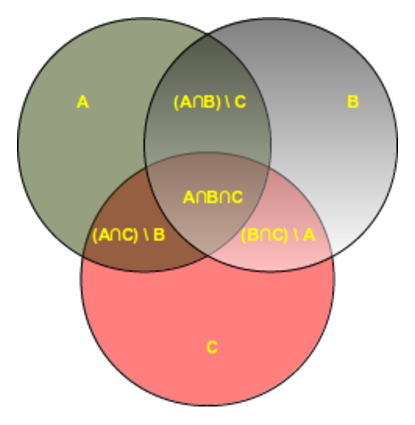
\includegraphics[width=0.8\textwidth]{sets_with_notations_back.eps}};
\end{tikzpicture}\\[8\baselineskip]
{\noindent {\Large\textsc{\textbf{halilović adis}}}}\\[\baselineskip]
}
\end{titlepage}

\newgeometry{right=2cm,top=5cm}
\hoffset -0.5cm
\thispagestyle{empty}
\pagecolor{mycol}
\newgeometry{left=1cm,right=5.5cm}
\begin{tikzpicture}[remember picture,overlay]
\draw [ultra thin, draw=black, fill=white, fill opacity=0.2	] ($(current page.north west)+(2cm,-2cm)$) rectangle  ($(current page.south east)+(-2cm,3cm)$) ;
\end{tikzpicture}

%\begin{tcolorbox}[colback=white]

\vspace{2cm}
\tableofcontents
\clearpage

\addtocontents{toc}{\vspace{5em}}
\addcontentsline{toc}{section}{sadržaj}
\addtocontents{toc}{\vspace{3em}}
\clearpage

\pagenumbering{arabic}

%\end{tcolorbox}
\restoregeometry
\pagecolor{white}

\newpage

\newgeometry{bottom=1in, top=1in,marginparwidth=1.8in,marginparsep=.25in}
\section{Skupovi}
\addtocontents{toc}{\vspace{1em}}
\reversemarginpar
\color{white}
\marginnote{\begin{tcolorbox}
\begin{flushleft}
\textbf{Skupovi su osnovni alat za učenje pa čak i za malu djecu. Kao bebe, oni nauče razlikovati "mene" od "mama" i "tata". Kao mališani nauče razlikovati i kategorisati objekte kao članove skupa po veličini, boji, ili obliku. TV emisija "Ulice sezama" uči djecu da prave skupove kroz igru. "Jedna od tih stvari je različita od ostalih."}
\end{flushleft}\end{tcolorbox}}[5cm]
\color{black}

\bigskip\bigskip
\Large{\lettrine{J}{} edan od osnovnih ljudskih nagona jeste da sortira i klasificira stvari. Razmislite, naprimjer. Koliko različitih skupova ste vi član? Ako krenete sa nekim jednostavnim kategorijama, kao jeste li muško ili žensko, vaša starosna grupa, država u kojoj živite. Tada ćete možda razmišljati i o etničkoj pripadnosti vaše porodice, sociološko-ekonomskoj grupi, nacionalnosti. Ovo su samo neke od mnogobrojnih načina kako bi mogli opisati sebe drugim ljudima.\par
Kakva je korist od ovakve kategorizacije? Kao što ćete vidjeti u nastavku ovog poglavlja, sortirajući stvari po skupovima pomaže vam organizirati i urediti vaš svijet. U mogućnosti ste da vladate velikim količinama informacija. Skupovi su učevni alat koji pomaže da se odgovori na pitanje: "Koje su karakteristike grupe?"\par
Skupovi postavljaju temelje ostalim matematičkim oblastima, poput logike i apstraktne algebre. Ustvari, knjiga \textit{El\' ements de Math\' ematique}, napisana od strane grupe francuskog matematičara pod pseudonimom "Nicolas Bourbaki", kaže: "U današnjici je moguće, logički govoreći: "U današnjici je moguće, logički rečeno, "}\\[\baselineskip]

\normalsize \subsection{Koncepti skupa}
\addtocontents{toc}{\vspace{1em}}
\bigskip\bigskip
Svakodnevno srešemo skupove u našim životima u raznim situacijama. Skup je kolekcija objekata, koji se nazivaju \textbf{elementi} ili \textbf{članovi} skupa. Naprimjer, Sjedinjena Američka država je kolekcija ili skup 50 manjih država. 50 pojedinih država su članovi ili elementi jednog skupa koji se naziva Sjedinjene Američke države.
Skup je \textbf{dobro definisan} ako se njegov sadržaj može jasno odrediti. Skup trenutnih sudija koji služe SAD vrhovnom sudu je dobro definisan skup jer njihovi članovi i sudije mogu biti imenovani. Skup tri najbolja auta nije dobro definisan skup jer riječ \textit{najbolji} različiti ljudi različito tumače. U ovom tekstu, mi koristimo samo dobro definisane skupove.\medskip

Za označavanje skupa obično se koriste sljedeće tri metode:
\begin{center}
\begin{itemize}
\item opis
\item popis ili obrazac
\item notacija skupa
\end{itemize}
\end{center}\medskip
Način označavanja skupa \textbf{opisom} prikazan je u primjeru 1.

\example{Opis skupova}{Napisati opis skupa koji sadrži elemente ponedjeljak, utorak, srijeda, četvrtak, petak, subota, nedjelja.}{Naziv skupa je "Dani u sedmici"}\medskip

\reversemarginpar
\color{white}
\marginnote{\begin{tcolorbox}
\begin{flushleft}
\textbf{Georg Cantor (1845-1918), rođen u St. Petersburg, Rusija, Poznat kao osnivač teorije skupova. Cantorov kreativni rad iz matematike umalo da bude izgubljen, kada je njegov otac insistirao da bude inžinjer a ne matematičar. Njegove dvije glavne knjige o teoriji skupova \textit{Foundations of General Theory of Aggregates} i \textit{Contributions to the Founding of the Theory of Transfinite Numbers}, izdate u 1883. i 1895., respektivno.}
\end{flushleft}\end{tcolorbox}}[9cm]
\color{black}

Smještanje elemenata skupa unutar velikih zagrada "$\{ \}$", naziva se ruster forma. Zagrade su bitan dio notacije jer ona označavaju članove skupa.\\
Naprimjer, $\{1, 2, 3\}$ predstavlja notaciju za skup kojem pripadaju elemnti 1, 2 i 3, ali $(1, 2, 3)$ i $[1, 2, 3]$ nisu skup iz razloga što velike i srednje zagrade n prikazuju skup.\medskip

Skupo se inače imenuju sa velikim štampanim slovima. Naprimjer, ime koje se obično bira za skup prirodnih brojeva je \textbf{N}.\\
\begin{tcolorbox}
\begin{center}
\textbf{\textsc{PRIRODNI BROJEVI}}\\
$N = \{1, 2, 3, 4, 5, ... \}$
\end{center}
\end{tcolorbox}\medskip

Tri tačke nakon 5, nazivaju se \textit{elipsa}, i označavaju da elementi skupa nastavljaju dalje na isti način. Ako se nakon elipse pojavi neki elemenat, znači da elementi idu na isti način sve do tog elementa uključujući i njega. Ovakva notacija prikazana je na primjeru 2b.\bigskip

\example{Skup u formi popisa}{Predstaviti sljedeće u formi popisa.\begin{enumerate}[label=\alph*),leftmargin=0.5cm]
\item Skup $A$ je skup prirodnih brojeva manjih od 4.
\item Skup $B$ je skup prirodnih brojeva manjih ili jednako 70.
\item Skup $P$ je skup planeta sunčevog sistema.
\end{enumerate}}{\begin{enumerate}[label=\alph*),leftmargin=0.5cm]
\item Prirodni brojevi manji od 4 su 1, 2 i 3. Prema tome, skup $A$ u formi popisa je $A=\{1,2,3\}$
\item $B=\{1, 2, 3, 4, ... , 70\}$. Broj 70 nakon 3 tačke znači da se brojevi nastavljaju na isti način sve do 70.
\item $P=\{$Merkur, Venera, Zemlja, Mars, Jupiter, Saturn, Uran, Neptun, Pluton$\}$.
\end{enumerate}}\bigskip

\example{Riječ \textit{uključujući}}{Sljedeće napiši u formi popisa.
\begin{enumerate}[label=\alph*),leftmargin=0.5cm]
\item Skup prirodnih brojeva između 5 i 8.
\item Skup prirodnih brojeva između 5 i 8, uključujući.
\end{enumerate}}{\begin{enumerate}[label=\alph*),leftmargin=0.5cm]
\item $A=\{6, 7\}$.
\item $B=\{5, 6, 7, 8\}$. Primjetite da riječ \textit{uključujuči} pokazuje na to da su i brojevi između 5 i 8 unutar skupa.
\end{enumerate}}\bigskip

Simbol \textbf{$\in$}, koji se čita, elemenat je, koristi se za označavanje članova u skupu. U primjeru 3, 6 je elemenat skupa A, pišemo $6\in A$. Također možemo napisati $6\in \{6, 7\}$. Isto tako $8\notin A$, što znači da 8 nije elemenat skupa A.

Notacija za kreiranje skupa (koja se ponekad naziva i notacija generatra skupa) može se koristiti da simbolizira skup. Navedena notacija skupa se često koristi u algebri. U nastavku primjer ilustrira njegov oblik.\smallskip

\begin{center}
\begin{pspicture}(0,0)(11,2.5)
%\psgrid(0,0)(11,2.5)
\rput(1,2){$D$}
\rput(2,1.967){$\textbf{=}$}
\rput(3,2){$\{$}
\rput(5,2){$\textbf{x}$}
\rput(7,2){$\textbf{|}$}
\rput(10,2){Uslov(i) $\}$}
\rput(1,1.5){$\uparrow$}
\rput(2,1.5){$\uparrow$}
\rput(3,1.5){$\uparrow$}
\rput(5,1.5){$\uparrow$}
\rput(7,1.5){$\uparrow$}
\rput(10,1.5){$\uparrow$}

\rput(1,0.7){Skup $D$}
\rput(2,0.7){je}
\rput(3,0.7){skup}
\rput(5,0.7){svih}
\rput(5,0.4){elemenata}
\rput(5,0.1){$x$}
\rput(7,0.7){takvih}
\rput(7,0.4){da}
\rput(10,0.7){$x$ zadovoljava uslove}
\rput(10,0.4){da bi bio dio skupa}
\end{pspicture}
\end{center}
\medskip

Uzmimo u obzir $E=\{x|x\in N$ i $x\>10\}$. Izraz se čita kao "Skup $E$ je skup svih elemenata x takvih da je x veće od 10." Uslovi koje $x$ mora ispuniti da bi bio elemenat skupa je $x\in N$, što znači da $x$ mora biti prirodan broj, i $x\> 10$, što znači da $x$ mora biti veće od 10. Brojevi koji ispunjavaju oba uvjeta su elementi skupa prirodnih brojeva većih od 10. Skup u formi popisa izgleda ovako
$$E=\{11, 12, 13, 14, ...\ \}$$

\example{Korištenje notacije za kreiranje skupova}{\begin{enumerate}[label=\alph*),leftmargin=0.5cm]
\item Napisati skup $B=\{1, 2, 3, 4, 5\}$ u obliku notacije za kreiranje skupa
\item Napiši, riječima, kako bi pročitao notaciju za kreiranje skupa $B$
\end{enumerate}}{\begin{enumerate}[label=\alph*),leftmargin=0.5cm]
\item Prema tome da se skup $B$ sastoji od prirodnih brojeva manjih od 6, pišemo $$B=\{x|x\in N\text { i } x< 6\}$$ Još jedan prihvatljiv odgovor je $B=\{x|x\in N$ i $x\leqslant 5\}$.
\item Skup $B$ je skup svih elemenata $x$ takvih da je $x$ prirodan broj i da je manji od 6.
\end{enumerate}}\medskip

\example{Forma popisa u notaciji građenja skupova}{\begin{enumerate}[label=\alph*),leftmargin=0.5cm]
\item Napisati skup $S = \{$Maine, Maryland, Massachusetts, Michigen, Minnesota, Mississippi, Missouri, Montana$\}$ u notaciji građenja skupova.
\item Napisati riječima kako bi pročitao/la skup $S$ u notaciji iz a).
\end{enumerate}}{\begin{enumerate}[label=\alph*),leftmargin=0.5cm]
\item $S=\{x|x$ je država u SAD-u čije ime počinje sa M$\}$.
\item Skup $S$ je skup svih elemenata x takvih da je x država SAD-a čije ime počinje sa slovom M.
\end{enumerate}}\medskip

\example{Notacija građenja skupova u formi popisa}{Napisati $A=\{x|x\in N$ i $2\leqslant x<8\}$ u formi popisa.}{$A=\{2, 3, 4, 5, 6, 7\}$}\medskip

Za skup se kaže da je \textbf{konačan}, ako ne sadrži elemente ili broj elemenata u skupu je prirodan broj. Skup $B=\{2, 4, 6, 8, 10\}$ je konačan skup zato što je broj elemenata skupa 5, a 5 je prirodan broj. Skup koji nije konačan naziva se \textbf{beskonačan} skup. Skup brojivih brojeva je jedan primjer beskonačnog skupa. O beskonačnim skupovima govorit ćemo u Poglavlju ...\par\smallskip
Još jedan bitan koncept jeste jednakost skupova.\smallskip

\reversemarginpar
\color{white}
\marginnote{\begin{tcolorbox}
\begin{flushleft}
\textbf{Učimo da grupišemo objekte prema onome što vidimo kao relevantne karakteristike razlikovanja. Jedan od načina na koji učitelji mjere ovu sposobnost jeste preko vizuelnih znakova.}
\end{flushleft}\end{tcolorbox}}
\color{black}

\begin{tcolorbox}
Skup $A$ \textbf{jendak} je skupu $B$, simbolično napisano $A=B$, ako i samo ako skup $A$ sadrži tačno iste elemente kao skup $B$.
\end{tcolorbox}\smallskip
\noindent Naprimjer, ako skup $A=\{1, 2, 3\}$ i skup $B=\{3, 1, 2\}$, onda $A=B$ zato što oba sadrže tačno iste elemente. Radoslijed elemenata u skupu nije bitan. Ako su dva skupa jednaka onda moraju oba biti sačinjnena od istog broja elemenata. Broj elemenata skupa naziva se \textit{osnovnu/kardinalni broj}.\smallskip
\begin{tcolorbox}
\textbf{Osnovni/Kardinanli broj} skupa $A$, simbolično napisanon$n(A)$, je broj elemenata skupa $A$.
\end{tcolorbox}\smallskip
Oba skupa $A=\{1, 2, 3\}$ i $B=\{$Engleska, Francuska, Japan$\}$ imaju osnovni/kardinalni broj 3; to jest, $n(A)=3$, i $n(B)=3$. Kažemo da skup $A$ i skup $B$ oba imaju kardinalnost 3.\par
Za dva skupa se kaže da su \textbf{ekvivalentna} ako oba posjeduju isti broj elemenata.\smallskip
\begin{tcolorbox}
Skup $A$ je \textbf{ekvivalentan} skupu $B$ ako i samo ako $n(A)=n(B)$.
\end{tcolorbox}\smallskip
\noindent Bilo koji skupovi koju su jednaki moraju biti i ekvivalenti. Međutim, nisu svi ekvivalentni skupovi jednaki. Skupovi $D=\{a, b, c\}$ i $E=\{$apple, orange, pear$\}$ su ekvivalenti, stoga što oba imaju isti osnovni/kardinalni broj, 3. Zbog toga što se elementi ralikuju, međutim, skupovi nisu jednaki.\par
Dva skupa koja su ekvivalentna i  imaju istu kardinalnost mogu se dopisati 1-1. Skup $A$ i skup $B$ mogu se dopisati 1-1 ako svaki elemenat skupa $A$ može biti povezan sa tačno jednim elementom skupa $B$ i svaki elemenat skupa $B$ može biti povezan sa tačno jednim elementom skupa $A$. Naprimjer, dopis 1-1 postoji između imena studenata sa liste razreda i sa njihovim identifikacionim brojevima zato što povezati njihova imena sa njihovim brojevima.\medskip

\begin{tcolorbox}
Uzmimo u obzir skup $B$, ime brenda produkta, i skup $D$, pića.
\begin{center}
$B=\{$Meggle, Biljana, Oaza, Zlatna džezva$\}$\\
$D=\{$čaj, mlijeko, kafa, voda$\}$
\end{center}
Dva zarličita dopisa 1-1 za skupove $B$ i $D$ slijede.\medskip
\begin{tcolorbox}[colback=white]
\smallskip
\begin{center}
\begin{pspicture}(0,0)(7,3)
%\psgrid(0,0)(7,3)
\rput(3.5,0){$D=\{$čaj, mlijeko, kafa, voda$\}$}
\rput(3.5,1){$B=\{$Meggle, Biljana, Oaza, Zlatna džezva$\}$}
\rput(3.5,2){$D=\{$čaj, mlijeko, kafa, voda$\}$}
\rput(3.5,3){$B=\{$Meggle, Biljana, Oaza, Zlatna džezva$\}$}

\psline[arrows=->](1.6,2.8)(2.25,2.2)%megle,čaj
\psline[arrows=->](2.85,2.8)(3.25,2.2)%biljana,mlijeko
\psline[arrows=->](4.05,2.8)(4.35,2.2)%oaza, kafa
\psline[arrows=->](5.7,2.8)(5.3,2.2)%z.dž, voda

\psline[arrows=->](1.6,0.8)(3.25,0.2)%done
\psline[arrows=->](2.85,0.8)(2.25,0.2)%done
\psline[arrows=->](4.05,0.8)(5.3,0.2)
\psline[arrows=->](5.7,0.8)(4.35,0.2)
\end{pspicture}
\smallskip
\end{center}
\end{tcolorbox}
\end{tcolorbox}
Drugi dopisi 1-1 su mogući između skupova $B$ i $D$. Da li znate koje piće ide sa kojim imenom brenda produkta?

\bigskip
\subsubsection{\textsc{nula ili prazan skup}}
\bigskip\bigskip
Neki skupovi ne sadrže ni jedan elemenat, kao naprimjer skup zebri koje su u ovoj sobi.\smallskip
\begin{tcolorbox}
Skup koji ne sadrži elemente naziva se \textbf{prazan skup} ili \textbf{nula skup} i simbolično se označava sa $\{\ \}$ ili $\varnothing$.
\end{tcolorbox}
Imajte na umu da ${\varnothing}$ nije prazan skup. Ovaj skup sadrži elemenat $\varnothing$ i ima kardinalnost 1. Skup $\{0\}$ također nije prazan skup zato što sadrži elemenat $0$. I on ima kardinalnost 1.\medskip

\example{Rješenja prirodnih brojeva}{Naznalite skup prirodnih brojeva koji zadovoljavaju jednačinu $x+2=0$.}{Vrijednosti koje zadovoljavaju jednačinu moraju biti takve da jednačina bude tačna. Samo broj $-2$ zadovoljava ovu jednačinu. Zbog toga što $-2$ nije prirodan bro, rješenje iove jednačine je $\{\ \}$ ili $\varnothing$.}

\subsubsection{\textsc{univerzalni skup}}
\addtocontents{toc}{\vspace{1em}}
\bigskip\bigskip
Još jedan bitan skup jeste \textbf{univerzalni skup}.\smallskip

\begin{tcolorbox}
\textbf{univerzalni skup}, simbolično napisan sa $U$, je skup koji sadrži sve elemente za bilo koju diskusiju.
\end{tcolorbox}\medskip

Kada je dat univerzalni skup, samo elementi univerzalnog skupa mogu se razmatrati prilikom rješavanja problema. Ako je, naprimjer, univerzalni skup za određeni problem definisan kao $U=\{1, 2, 3, 4, .., 10\}$, onda samo prirodni brojevi od 1 do 10 mogu biti korišteni tokom problema.

\vspace{2cm}
\begin{tcolorbox}[title=\textbf{ZADACI ZA VJEŽBU}]
\begin{minipage}{0.5\textwidth}
\textbf{KONCEPT/VJEŽBE PISANJA}\\
\textit{U zadacima od 1 do 8, odgovoriti na pitanja punom rečenicom.}
\begin{enumerate}
\item Šta je skup?
\item Koje su tri varijante kojima skup može biti zapisan? navedite primjer za svaku od njih.
\item Šta je beskonačan skup?
\item Šta je konačan skup?
\item Šta su jednaki skupovi?
\item Šta su ekvivalenti skupovi?
\item Šta je kardinalni broj skupa?
\item Šta je univerzalni skup?
\item Šta je prazan skup?
\end{enumerate}
\textbf{ZADACI ZA VJEŽBU VJEŠTINE}\\
\textit{U zadacima od 10 do 12, odredite da li su skupovi dobro definisani.}
\begin{enumerate}
\setcounter{enumi}{9}
\item Skup najboljih internet sajtova
\item Skup ljudi koji posjeduju velike pse
\item Skup učenika razreda koji su rođeni u Bosni i Hercegovini
\end{enumerate}
\end{minipage}
\begin{minipage}{0.5\textwidth}
\textit{U zadacima od 13 do 17, odredite da li je skup konačan ili beskonačan}.
\begin{enumerate}
\setcounter{enumi}{12}
\item $\{1, 3, 5, 7, ...\}$
\item Skup parnih brojeva većih od 15
\item Skup neparnih brojeva većih od 15
\item Skup vrabaca koji cvrkuću u parku 4. jula u 10 sati.
\item Skup umnožaka sa 6 između 0 i 60
\end{enumerate}
\textit{U zadacima od 18 do 22, navedene skupove pretstaviti u formi popisa}.
\begin{enumerate}
\setcounter{enumi}{17}
\item Skup kontinenata svijeta
\item Skup prirodnih brojeva između 10 i 178
\item $B=\{x|x\in N$ i $x$ je paran$\}$
\item $C=\{x|x+6=10\}$
\item $D=\{x|x\in N$ i $6\leqslant x < 72\}$
\end{enumerate}
\textit{U zadacima od 22 do x, navedene skupove pretstaviti u notaciji kreiranja skupova}.
\begin{enumerate}
\setcounter{enumi}{22}
\item $A=\{1, 2, 3, 4, 5, 6, 7, 8, 9\}$
\item $B=\{4, 5, 6, 7, 8\}$
\item $C=\{3, 6, 9, 12, ...\}$
\end{enumerate}
\end{minipage}
\end{tcolorbox}
\addcontentsline{toc}{section}{zadaci za vježbu 1.1}
\addtocontents{toc}{\vspace{1em}}

\newpage
\subsection{Podskupovi}
\addtocontents{toc}{\vspace{1em}}
\bigskip\bigskip
U našem složenom svijetu, inače veće skupove razbijamo na manje skupove s kojim nam je lakše raditi. takve skupove nazivamo \textit{podskupovi}. Napriimjer, uzmite u obzir skup ljudi u vašem odjeljenju. Prepostavimo da kategorišemo ljude po prvom slovu njihovog prezimena(A, B, C, idt.). Kada to odradimo, svaki od novih skupova može se smatrati podskupom orginalnog skupa. Svaki od ovih podskupova može se dalje  razdvajati. Naprimjer, osobe kod kojih prezime počinje sa A možemo kategorisati po tome jesu li muškog ili ženskog spola ili po njihovim godinama. Svaka od ovih kolekcija je podskup. Početni skup može imati mnogo različitih podskupova.\smallskip

\begin{tcolorbox}
Skup $A$ je \textbf{podskup} skupa $B$, simbolično pišemo $A\subseteq B$, ako i samo ako su elementi skupa $A$ takožer elementi skupa $B$.
\end{tcolorbox}\medskip

Simbol $A\nsubseteq B$ označava da "skup je $A$ podskup skupa $B$". Simbol $\nsubseteq$ znači "nije podskup". Iz toga, $A\nsubseteq B$ znači da skup $A$ nije podskup skupa $B$. \textit{Da pokažemo to da skup $A$ nije podskup skupa $B$, moramo pronaći makar jedan elemenat skupa $A$ koji nije elemenat skupa $B$.}\medskip

\reversemarginpar
\color{white}
\marginnote{\begin{tcolorbox}
\begin{flushleft}
\textbf{Većinu duga što vidimo su primarne duge, ali dese se momenti kada na sekundu, možemo vidjeti blijedu dugu iza prve. U ovoj drugoj dugi, redoslijed boja je izvrnut. Obje duge sadrže isti skup boja, pa je svaka od boja podksup jedna drugoj.}
\end{flushleft}\end{tcolorbox}}[7cm]
\color{black}

\example{Da li je $A$ podskup?}{Odrediti da li je skup $A$ podskup skupa $B$.
\begin{enumerate}[label=\alph*),leftmargin=0.5cm]
\item $A=\{$krastavac, paradajz, paprika$\}$
$B=\{$paradajz, sir, krastavac, paprika$\}$
\item $A=\{2, 3, 4, 5\}$\quad $B=\{2, 3\}$
\item $A=\{x|x$ žuto voće$\}$
$B=\{$ crveno voće$\}$
\item $A=\{$kašika, viljuška, nož$\}$
$B=\{$nož, kašika, viljuška$\}$
\end{enumerate}}{%
{\begin{enumerate}[label=\alph*),leftmargin=0.5cm]
\item Svi elementi skupa $A$ sadržani su u skupu $B$, prema tome $A\subseteq B$.
\item Elementi 4 i 5 su u skupu $A$ ali ne u skupu $B$, stoga $A\nsubseteq B$ ($A$ nije podskup od $B$). Mežutim, u ovom primjeru svi elementi skupa $B$ sadržani su u skupu $A$; stoga, $B\subseteq A$.
\item Postoji voće, kao naprimjer banane, koje su iz skupa $A$ ali ne iz skupa $B$,pa $A\nsubseteq B$.
\item Svi elementi skupa $A$ sadržani su u skupu $B$, prema tome $A\subseteq B$. Primjetite da je $A=$ skup $B$.
\end{enumerate}}}

\subsubsection{\textsc{odgovarajući podskupovi}}
\bigskip\bigskip
\begin{tcolorbox}
Skup $A$ je \textbf{odgovarajući podskup} skupa $B$, simbolično pišemo $A\subset B$, ako i samo ako su svi elementi skupa $A$ također elementi skupa $B$ i skup $A\neq$ skup $B$(to jest, skup $B$ mora imati makar jedan elemenat koji se ne nalazi u skupu $A$).
\end{tcolorbox}\smallskip

Uzmite u obzir da $A=\{$crvena, plava, žuta$\}$ i $B=\{$crvena, narandžasta, žuta, zelena, plava, ljubičasta$\}$. Skup $A$ je \textit{podskup} skupa $B$, $A\subseteq B$, zato što je svaki elemenat skupa $A$ također elemenat skupa $B$. Skup $A$ je također \textit{odgovarajući skup} skupa $B$, $A\subset B$, zato šsto skup $A$ i skup $B$ nisu jednaki. Sada uzmimo u obzir skup $C=\{$auto, autobus, voz$\}$ i skup $D=\{$voz, auto, autobus$\}$. Skup $C$ je podskup skupa $D$, $C\subseteq D$, zato što je svaki elemenat skupa $C$ također elemenat skupa $D$. Međutim, skup $C$, nije odgovarajući podskup skupa $D$, $C\not\subset D$, zato što su skup $C$ i skup $D$ jednaki skupovi.\bigskip

\example{Da li je skup odgovarajući podskup?}{Odrediti da li je skup $A$ odgovarajući podskup skupa $B$.
\begin{enumerate}[label=\alph*),leftmargin=0.5cm]
\item $A=\{$Korveta, Vajper, BMW$\}$
$B=\{$Vajper, BMW, Kamero, Korveta, Mustang$\}$
\item $A=\{a, b, c, d\}$\quad $B=\{a, c, b, d\}$
\end{enumerate}}{\begin{enumerate}[label=\alph*),leftmargin=0.5cm]
\item Svi elementi skupa $A$ su sadržani u skupu $B$ i $B$ nisu jednaki; iz toga slijedi, $A\subset B$.
\item Skup $A=$ skup $B$, prema tome $A\not\subset B$. (Međutim, $A\subseteq B.$)
\end{enumerate}}\bigskip

Svaki skup je podskup samoga sebe, ali nijedan skup nije odgovarajući podskup sebe. Za sve skupove $A$, $A\subseteq A$, ali $A\not\subset A$. Naprimjer, ako  $A=\{1, 2, 3\}$, onda $A\subseteq A$ zato što je svaki elemenat skupa $A$ sadržan u skupu $A$, ali $A\not\subset A$ zato što je skup $A=$ skupu $A$.\par
Neka $A = \{\ \}$ i $B=\{1, 2, 3, 4\}$. Da li je $A\subseteq B$? Da bi poakazali $A\nsubseteq B$, treba pronaći makar jedan elemenat skupa $A$ koji nije elemenat skupa $B$. pošto ovo ne može biti odrađeno, $A\subseteq B$ mora biti tačno. Korsteći se istim rezonom, možemo pokazati da \textit{prazan  skup je podskup svih skupova, uključujući i samoga sebe.}

\example{Elemenat ili podskup?}{\begin{minipage}{\textwidth}
Odredite da li su sljedeći izrazi tačni.
\end{minipage}\\

\begin{minipage}{0.5\textwidth}
\begin{enumerate}[label=\alph*),leftmargin=0.5cm]
\item $3\in\{3, 4, 5\}$
\item[c)] $\{3\}\in \{\{3\}, \{4\}, \{5\}\}$
\item[e)] $3\subseteq \{3, 4, 5\}$
\end{enumerate}
\end{minipage}\begin{minipage}{0.5\textwidth}
\begin{enumerate}[label=\alph*),leftmargin=0.5cm]
\item[b)] $\{3\}\in \{3, 4, 5\}$
\item[d)] $\{3\}\subseteq \{3, 4, 5\}$
\item[f)] $\{\ \}\subseteq \{3, 4, 5\}$
\end{enumerate}
\end{minipage}}{\begin{enumerate}[label=\alph*),leftmargin=0.5cm]
\item $3\in \{3, 4, 5\}$ je tačan izraz zato što je 3 član skupa $\{3, 4, 5\}$.
\item $\{3\}\in \{3, 4, 5\}$ je netačan izraz zato što je $\{3\}$ skup, a skup $\{3\}$ nije elemenat skupa $\}3, 4, 5\}$.
\item $\{3\}\in \{\{3\}, \{4\}, \{5\}\}$ je tačan izraz zato što je $\{3\}$ elemenat skupa. Elementi skupa $\{\{3\}, \{4\}, \{5\}\}$ su sami sobom skupovi.
\item $\{3\}\subseteq \{3, 4, 5\}$ je tačan izraz zato što je svaki elemenat prvog skupa ujedno elemenat drugog skupa.
\item $3\subseteq \{3, 4, 5\}$ je netačan izraz zato što 3 nije u velikim zagradama, pa nije skup i prema tome ne može biti podksup. 3 je elemenat skupa kako je naglašeno u dijelu a).
\item $\{\ \}\subseteq \{3, 4, 5\}$ je tačan izraz zato što je prazan skup podskup svakog skupa.
\end{enumerate}}

\subsubsection{\textsc{broj podskupova}}
\addtocontents{toc}{\vspace{1em}}
\bigskip\bigskip
Koliko se različitih podskupova može napraviti od jednog ponuđenog skupa? Prazan skup nema elemenata i ima tačno jedan podskup. A skup sa tri elementa ima osam podskupova. Pogledajte tabelu 1 na strani 10. koliko podskupova sadrži skup sa četiri elementa?\medskip

\begin{table}[h]
\Large
\centering
\begin{tabular}{lll}
\hline
\textbf{Skup} & \textbf{Podskup}                                                                                                 & \textbf{Broj podskupova}     \\ \hline
$\{ \}$         & $\{ \}$                                                                                                            & $1=2^0$       \\ \hline
$\{a\}$         & \begin{tabular}[c]{@{}l@{}}$\{a\}$\\ $\{ \}$\end{tabular}                                                            & $2=2^1$       \\ \hline
$\{a, b\}$      & \begin{tabular}[c]{@{}l@{}}$\{a, b\}$\\ $\{a\}, \{b\}$\\ $\{ \}$\end{tabular}                                          & $4=2\times 2=2^2$   \\ \hline
$\{a, b, c\}$   & \begin{tabular}[c]{@{}l@{}}$\{a, b, c\}$\\ $\{a, b\}, \{a, c\}, \{b, c\}$\\ $\{a\}, \{b\}, \{c\}$\\ $\{ \}$\end{tabular} & $8=2\times 2\times 2=2^3$ \\ \hline
\end{tabular}
\caption{Broj podskupova}
\end{table}

Nastavljajuči ovu tabelu sa većim i većim skupovima, možemo razviti generalnu formulu za računanje broja različitih podskupova datog skupa.

\begin{tcolorbox}
\textbf{Broj različitih skupova} konačnog skupa $A$ je $2^n$m gdje $n$ predstavlja broj elemenata skupa $A$.
\end{tcolorbox}\smallskip

\reversemarginpar
\color{white}
\marginnote{\begin{tcolorbox}
\begin{flushleft}
\textbf{\textbf{\textit{Sa sedam različitih}} pločica sa slovima, postoji 5040 različitih načina da poredamo pločice. Četiri slova S, L, E, D mogu biti poredani u 24 različita načina.}
m\end{flushleft}\end{tcolorbox}}[6cm]
\color{black}

\example{Različiti podskupovi}{\begin{enumerate}[label=\alph*),leftmargin=0.5cm]
\item Odredite broj različitih podskupova skupa $\{$S, L, E, D$\}$.
\item Napiđite sve raličite podskupove skupa $\{$S, L, E, D$\}$.
\item Koliko različitih podskupova su pravilni podskupovi?
\end{enumerate}}{\begin{enumerate}[label=\alph*),leftmargin=0.5cm]
\item Broj elemenata skupa je 4, prema tome, broj različitih skupova je $2^4=2\times 2 \times 2 \times 2=16$.
\item \begin{tabular}[t]{lllll}
$\{S, L, E, D\}$ & $\{S, L, E\}$ & $\{S, L\}$ & $\{S\}$ & $\{ \}$ \\
               & $\{S, L, D\}$ & $\{S, E\}$ & $\{L\}$ &       \\
               & $\{S, E, D\}$ & $\{S, D\}$ & $\{E\}$ &       \\
               & $\{L, E, D\}$ & $\{L, E\}$ & $\{D\}$ &       \\
               &             & $\{L, D\}$ &       &       \\
               &             & $\{E, D\}$ &       &      
\end{tabular}
\item Pravilnih podskupova ima 15. Svi podskupovi osim $\{S, L, E, D\}$ su pravilni podskupovi.
\end{enumerate}}\medskip

\begin{tcolorbox}[title=\textbf{ZADACI ZA VJEŽBU}]
\begin{minipage}{0.5\textwidth}
\textbf{KONCEPT/VJEŽBE PISANJA}\\
\textit{U zadacima od 1 do 6, odgovoriti na pitanja punom rečenicom.}
\begin{enumerate}
\item Šta je podskup?
\item Šta je pravilan podskup?
\item Objasni razliku između podskupa i pravilnog podksupa.
\item Koja je formula za određivanje različitog broja podskupova za skup sa $n$? različitih elemenata?
\item Koja je formula za određivanje različitog broja pravilnih podskupova za skup sa $n$? različitih elemenata?
\item Je li može bilo koji skup biti pravilan podskup samoga sebe? Objasni.
\end{enumerate}
\textbf{ZADACI ZA VJEŽBU VJEŠTINE}\\
\textit{U zadacima od 7 do 24, odgovorite sa tačno ili netačno. Ako je netačno, obrazloži.}
\begin{enumerate}
\setcounter{enumi}{7}
\item $\{\ \}\in \{1, 2, 3, 4\}$
\end{enumerate}
\end{minipage}
\begin{minipage}{0.5\textwidth}
\begin{enumerate}
\setcounter{enumi}{8}
\item $\{\ \}\subseteq \{$Asim, Nikola, Zdenko$\}$
\item crvena$\subset \{$crvena, zelena, plava$\}$
\item 5$\not\in \{2,4,6\}$
\item $\{$Petar, Amela, Malik$\}\subseteq \{$Amela, Katarina, Brijana$\}$
\item $\{\ \}=\{\varnothing \}$
\item $\{1\}\subseteq \{1, 9, 5\}$
\item $\varnothing =\{\ \}$
\item $0=\{\ \}$
\item $\{0\}=\varnothing$
\item $\{1, 5, 9\}\subseteq \{1, 9, 5\}$
\item $\{5\}\in \{5, 6, 7\}$
\item $\{3, 5, 9\}\not\subset \{3, 9, 5\}$
\item $\{\ \}\subset \{\ \}$
\item $\{1\}\in \{\{1\}, \{2\}, \{3\}\}$
\item $\{b, a, t\}\subseteq \{t, a, b\}$
\end{enumerate}
\end{minipage}
\end{tcolorbox}
\addcontentsline{toc}{section}{zadaci za vježbu 1.2}
\addtocontents{toc}{\vspace{3em}}

\newpage
\section*{\textbf{Literatura}}
\hrule
\bigskip\bigskip
%\begin{tcolorbox}
\large
\begin{enumerate}
\item A Survey Of Mathematics With Applications (ANGEL PORTER)
\item StackExchange (https://tex.stackexchange.com)
\item Overleaf (https://www.overleaf.com)
\item texblog (https://texblog.org/)
\item stackoverflow (https://stackoverflow.com)
\item \LaTeX 4technics (https://www.latex4technics.com/)
\item CTAN Comprehensive \TeX Archive Network (CTAN Comprehensive \TeX Archive Network)
\item Share\LaTeX (https://sharelatex.psi.ch)
\item LaTeX Community - Latex.org (https://latex.org)
\item http://www.emerson.emory.edu
\end{enumerate}
%\end{tcolorbox}

\addcontentsline{toc}{section}{literatura}

\end{document}